\documentclass{article}
\usepackage[dvipsnames]{xcolor}
\usepackage{tikz}
\usepackage{tikzpeople}
\definecolor{nhs-green}{RGB}{0,103,71}
\definecolor{nhs-blue}{RGB}{0,94,184}
\begin{document}

\begin{tikzpicture}
\definecolor{myskin}{named}{Tan};

	\tikzset{		myskin/.style=        {color=myskin,top color=myskin!70, bottom color=myskin,shading angle=45}}
	
\node[mexican,minimum size=2.5cm] (M) at (0pt,-250pt) {A
Mexican};
\draw[myskin]
  (-60.0pt,-60.0pt) .. controls (-56pt,-64pt) and (-53pt,-68pt)..
  (-40pt,-68pt) .. controls (-40pt,-80pt)  and (-40pt,-90pt)..
  (-30pt,-110pt) .. controls (0pt,-120pt) and (30pt,-110pt) ..
  ( 30pt,-110pt) .. controls (40pt,-90pt)  and (40pt,-80pt)..
  (40pt,-68pt) .. controls (53pt,-68pt) and (56pt,-64pt)..
  ( 60pt,-60pt) .. controls ( 50pt, 0pt) and (-50pt, 0pt) .. 
		(-60pt,-60pt) -- cycle;
 %%%%%%%%%%%% The following lacks proportion%%%%%%%%%%%
  % \draw[myskin]
  % (-60.0pt,-60.0pt) .. controls (-56pt,-64pt) and (-53pt,-68pt)..
  % (-40pt,-68pt) .. controls (-40pt,-80pt)  and (-40pt,-90pt)..
  % (-30pt,-100pt) .. controls (0pt,-110pt) and (30pt,-100pt) ..
  % ( 30pt,-100pt) .. controls (40pt,-90pt)  and (40pt,-80pt)..
  % (40pt,-68pt) .. controls (53pt,-68pt) and (56pt,-64pt)..
  % ( 60pt,-60pt) .. controls ( 50pt, 0pt) and (-50pt, 0pt) .. 
		% (-60pt,-60pt) -- cycle;
  %%%%%%%%%%%%%%%%%%%%%%%%%%%%%%%%%%%%%%%%%%%%%%%%%%%%%%%%

  \draw[myskin] (0pt,0pt) ellipse (30pt and 27pt);
% \draw[fill=white](0pt,-50pt) ellipse (18pt and 13pt);
% \clip (0pt,-50pt) ellipse (16pt and 12pt) node {\includegraphics[width=.11\textwidth]{flags/in.png}};

\draw[fill=white](0pt,-60pt) circle (20pt);
\clip (0pt,-60pt) circle (19pt) node {\includegraphics[width=.12\textwidth]{flags/indianflag.png}};

 
% \node[inner sep=0pt] (russell) at (0pt,-60pt) {\includegraphics[width=.08\textwidth]{flags/mx.png}};
\end{tikzpicture}
\newpage

\begin{tikzpicture}
\definecolor{myskin}{named}{blue};

	\tikzset{		myskin/.style=        {color=myskin,top color=myskin!70, bottom color=myskin,shading angle=45}}
	
\node[builder,minimum size=2.5cm] (M) at (0pt,-250pt) {A
Builder};
  \draw[myskin]
  (-60.0pt,-60.0pt) .. controls (-56pt,-64pt) and (-53pt,-68pt)..
  (-40pt,-68pt) .. controls (-40pt,-80pt)  and (-40pt,-90pt)..
  (-30pt,-110pt) .. controls (0pt,-120pt) and (30pt,-110pt) ..
  ( 30pt,-110pt) .. controls (40pt,-90pt)  and (40pt,-80pt)..
  (40pt,-68pt) .. controls (53pt,-68pt) and (56pt,-64pt)..
  ( 60pt,-60pt) .. controls ( 50pt, 0pt) and (-50pt, 0pt) .. 
		(-60pt,-60pt) -- cycle;
  \draw[myskin] (0pt,0pt) ellipse (30pt and 27pt);
% \draw[fill=white](0pt,-50pt) ellipse (18pt and 13pt);
% \clip (0pt,-50pt) ellipse (16pt and 12pt) node {\includegraphics[width=.11\textwidth]{flags/in.png}};


\draw[fill=white](0pt,-60pt) circle (20pt);
\clip (0pt,-60pt) circle (19pt) node {\includegraphics[width=.09\textwidth]{labour.png}};


 
%\node[inner sep=0pt] (russell) at (0pt,-55pt) {\includegraphics[width=.08\textwidth]{labour.png}};
\end{tikzpicture}
\newpage

\begin{tikzpicture}
\definecolor{myskin}{named}{nhs-blue};
%MidnightBlue
	\tikzset{		myskin/.style=        {color=myskin,top color=myskin!70, bottom color=myskin,shading angle=45}}
	
\node[physician,female,minimum size=2.5cm] (M) at (0pt,-250pt) {A
Doctor};
  \draw[myskin]
  (-60.0pt,-60.0pt) .. controls (-56pt,-64pt) and (-53pt,-68pt)..
  (-40pt,-68pt) .. controls (-40pt,-80pt)  and (-40pt,-90pt)..
  (-30pt,-110pt) .. controls (0pt,-120pt) and (30pt,-110pt) ..
  ( 30pt,-110pt) .. controls (40pt,-90pt)  and (40pt,-80pt)..
  (40pt,-68pt) .. controls (53pt,-68pt) and (56pt,-64pt)..
  ( 60pt,-60pt) .. controls ( 50pt, 0pt) and (-50pt, 0pt) .. 
		(-60pt,-60pt) -- cycle;
  \draw[myskin] (0pt,0pt) ellipse (30pt and 27pt);
% \draw[fill=white](0pt,-50pt) ellipse (18pt and 13pt);
% \clip (0pt,-50pt) ellipse (16pt and 12pt) node {\includegraphics[width=.11\textwidth]{flags/in.png}};


\draw[fill=white](0pt,-55pt) circle (18pt);
\clip (0pt,-55pt) circle (17pt) node {\includegraphics[width=.07\textwidth]{doctor2.png}};


 
%\node[inner sep=0pt] (russell) at (0pt,-55pt) {\includegraphics[width=.08\textwidth]{labour.png}};
\end{tikzpicture}


\newpage

\begin{tikzpicture}
\definecolor{myskin}{named}{nhs-green};


	\tikzset{		myskin/.style=        {color=myskin,top color=myskin!70, bottom color=myskin,shading angle=45}}
	
\node[nurse,female,minimum size=2.5cm] (M) at (0pt,-250pt) {A
Nurse};
  \draw[myskin]
  (-60.0pt,-60.0pt) .. controls (-56pt,-64pt) and (-53pt,-68pt)..
  (-40pt,-68pt) .. controls (-40pt,-80pt)  and (-40pt,-90pt)..
  (-30pt,-110pt) .. controls (0pt,-120pt) and (30pt,-110pt) ..
  ( 30pt,-110pt) .. controls (40pt,-90pt)  and (40pt,-80pt)..
  (40pt,-68pt) .. controls (53pt,-68pt) and (56pt,-64pt)..
  ( 60pt,-60pt) .. controls ( 50pt, 0pt) and (-50pt, 0pt) .. 
		(-60pt,-60pt) -- cycle;
  \draw[myskin] (0pt,0pt) ellipse (30pt and 27pt);
% \draw[fill=white](0pt,-50pt) ellipse (18pt and 13pt);
% \clip (0pt,-50pt) ellipse (16pt and 12pt) node {\includegraphics[width=.11\textwidth]{flags/in.png}};


\draw[fill=white](0pt,-55pt) circle (18pt);
\clip (0pt,-55pt) circle (17pt) node {\includegraphics[width=.07\textwidth]{nurse.png}};


 
%\node[inner sep=0pt] (russell) at (0pt,-55pt) {\includegraphics[width=.08\textwidth]{labour.png}};
\end{tikzpicture}
\end{document}

\documentclass{article}
\usepackage{tikz}
\begin{document}
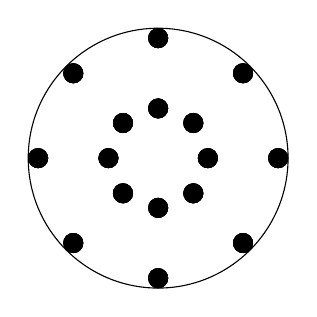
\begin{tikzpicture}
    \draw[fill=white] (0,0) circle (1.65);
    
    \foreach \x in {0,45,...,315}
        \foreach \y in {22.5,67.5,...,337.5}
            \draw[fill=black] ({1.65*cos(\x)*sin(\y)}, {1.65*sin(\x)*sin(\y)}) circle (0.12);
\end{tikzpicture}
\end{document}